\documentclass[
	letterpaper, % Paper size, specify a4paper (A4) or letterpaper (US letter)
	10pt, % Default font size, specify 10pt, 11pt or 12pt
]{CSUniSchoolLabReport}

%----------------------------------------------------------------------------------------
%	REPORT INFORMATION
%----------------------------------------------------------------------------------------

\title{Creating and Combining Sinusoids in MATLAB \\ Circuits \& Signals \\ EECE2150} % Report title

\author{Michael \textsc{Brodskiy}}

\date{February 23, 2023} % Date of the report

%----------------------------------------------------------------------------------------


\begin{document}

\maketitle % Insert the title, author and date using the information specified above

\begin{center}
	\begin{tabular}{l r}
		Date Performed: & February 16, 2023 \\ % Date the experiment was performed
        Partner: & Juan \textsc{Zapata} \\ % Partner names
		Instructor: & Professor \textsc{Sun} % Instructor/supervisor
	\end{tabular}
\end{center}

\setcounter{section}{-1}

\section{Introduction}

The purpose of this laboratory experimentation is to familiarize oneself with the concept of sinusoids, as well as developing them in MATLAB. By integrating MATLAB and sinusoid construction together, the knowledge gained may be applied to alternating current circuits.

\subsection{Q1} In both formulas, $x(t)=A\sin(\omega t+\theta)=A\sin(2\pi ft+\theta)$, the value within the $\sin$ parameters are radian values because $\omega$ is the angular frequency, measured in radians per second, multiplying it by seconds obtains simply radians, which are added to the phase shift value $\theta$, also measured in radians. Thus, the first formula correctly uses radians. In the second formula, $2\pi$ has units of radians, $f$ has units of Hertz, or inverse seconds, and $t$ has units of seconds. Multiplying these together, units of radians are once again obtained, and subsequently added to the phase shift value.

\section{Part I}

\subsection{Q2} $F=\frac{1}{16}$ cycles per sample, which means there are 16 samples per cycle.

\subsection{Q3} Changing the phase value to .5 shifts the graph to the left by .5 radians.

\subsection{Q4} There is no major difference in the sound; rather, the difference is in that the sound starts from a different point.

\subsection{Q5} Due to the decreased amplitude, the sound seems to be a bit quieter than it was before.

\subsection{Q6} It seems that, as the sampling frequency decreases, the quality of the blocks decreases as well; they blocks appear to shift from solid to rectangles to triangles.

\subsection{Q7} As the sampling frequency decreases, it seems that the quality and pitch of the sound are simultaneously decreasing. This could be because it samples less, so it produces a less precise sound.

\section{Part II}

\subsection{Q8} $A$ controls the amplitude of the sinusoid.

\begin{figure}[H]
  \centering
  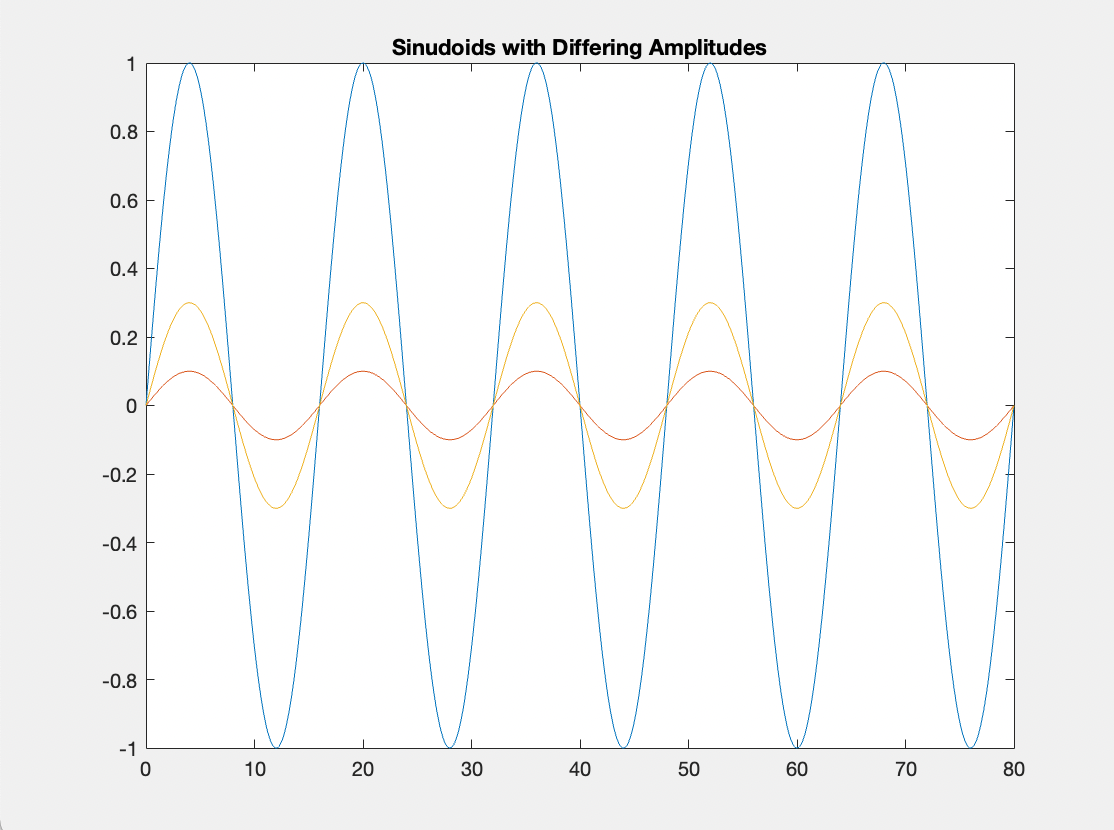
\includegraphics[width=.9\textwidth]{Figures/L7Ampl.png}
  \caption{Varying $A$ values for sinusoids}
  \label{fig:1}
\end{figure}

\subsection{Q9} The sinusoids all seem to have a phase difference, as they are shifted over to the left by the phase shift value.

\begin{figure}[H]
  \centering
  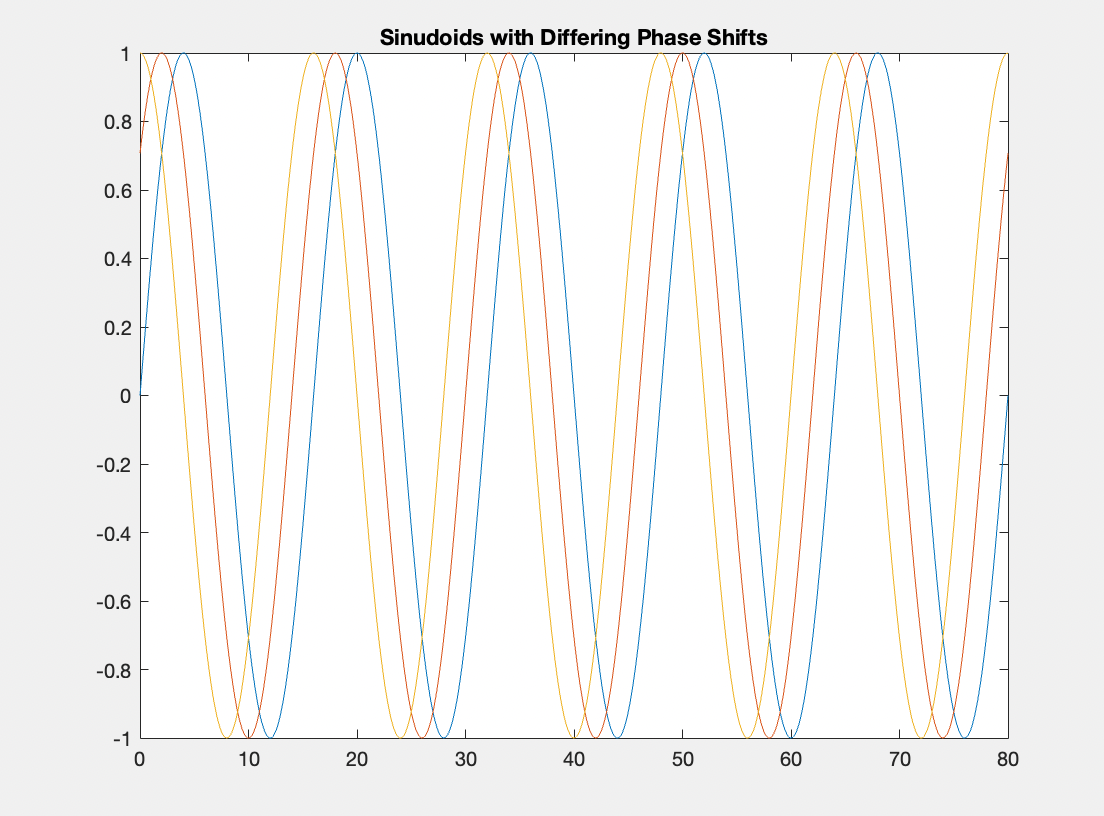
\includegraphics[width=.9\textwidth]{Figures/L7PS1.png}
  \caption{All of the sinusoids are shifted to the left by their phase shift value}
  \label{fig:2}
\end{figure}

\subsection{Q10} The graphs for the 0 and $4\pi$ phase shifts are identical, as $4\pi$ is an integer multiple of $2\pi$, meaning that it returns to the same state as if the phase shift had been 0.

\begin{figure}[H]
  \centering
  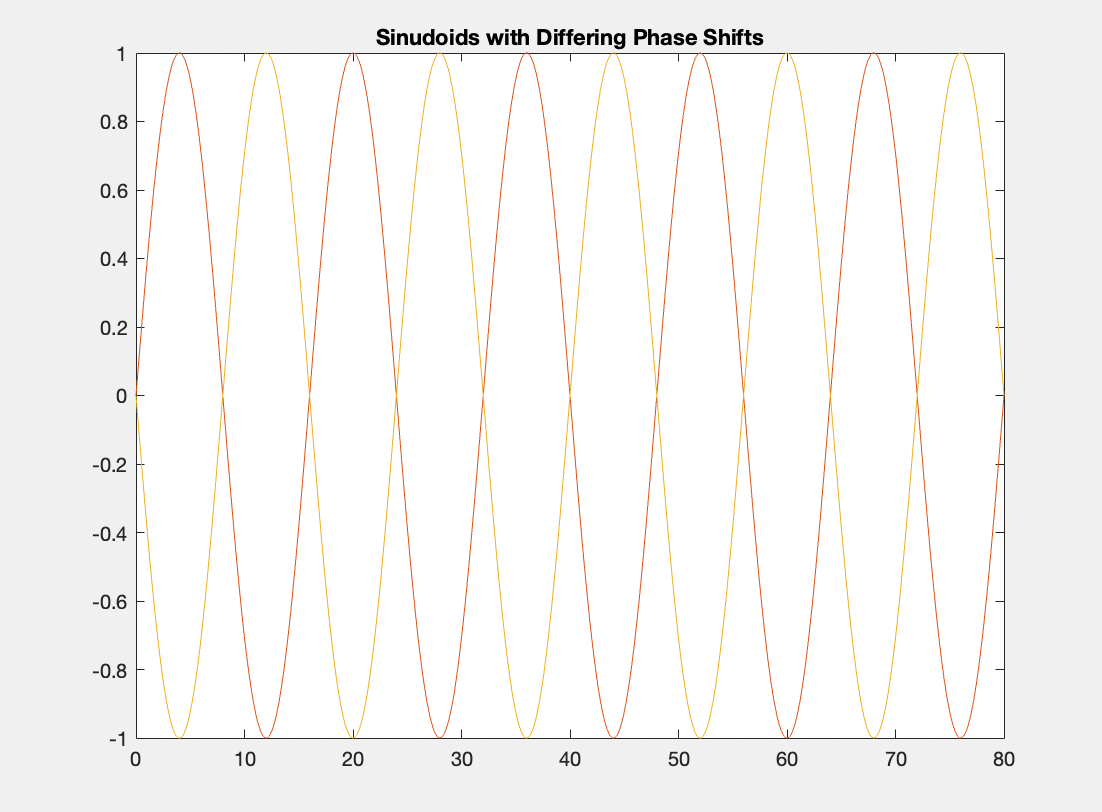
\includegraphics[width=.9\textwidth]{Figures/L7PS2.png}
  \caption{Phase shifts $0$ and $4\pi$ are overlayed}
  \label{fig:3}
\end{figure}

\subsection{Q11} The sound of the sinusoid is not influenced by the phase change; rather, all that changes is that the noise at which the sinusoid begins is different.

\section{Part III}

\subsection{Q12} The waveform seems to have more ``interference''; that is, it appears that the peaks become more bumpy with each added sinusoid. The number of peaks is equal to the amount of sinusoids summed.

\begin{figure}[H]
  \centering
  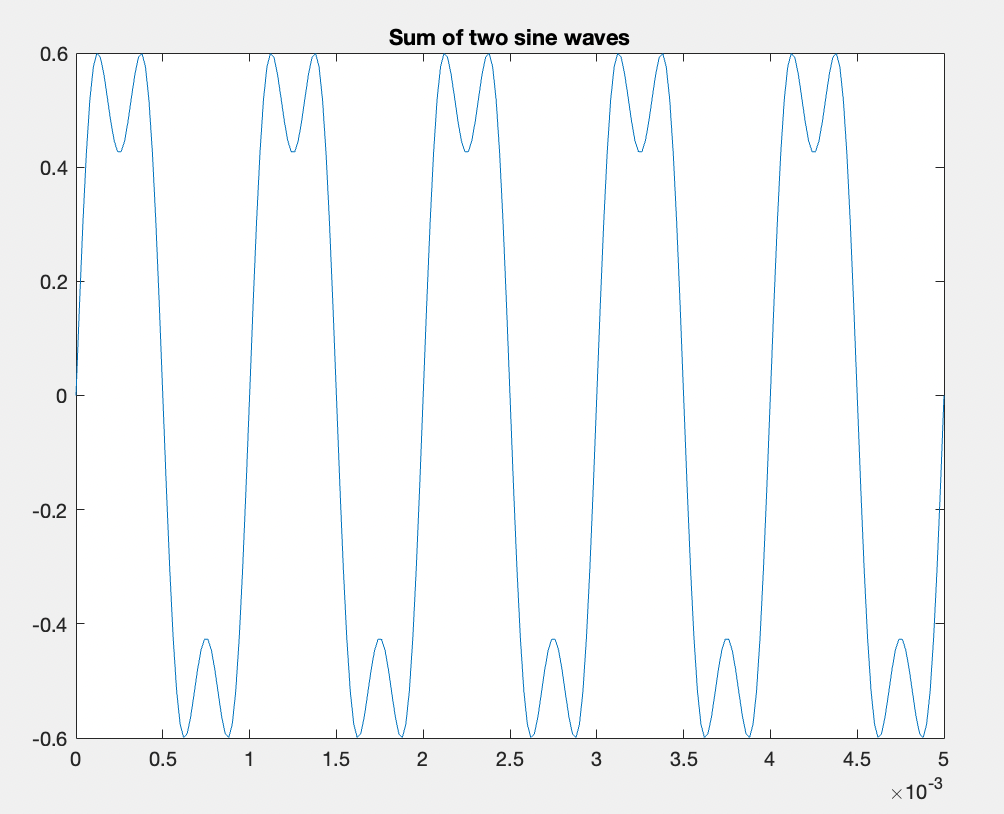
\includegraphics[width=.9\textwidth]{Figures/L7Sum1.png}
  \caption{Summing $n=1,2$}
  \label{fig:4}
\end{figure}

\begin{figure}[H]
  \centering
  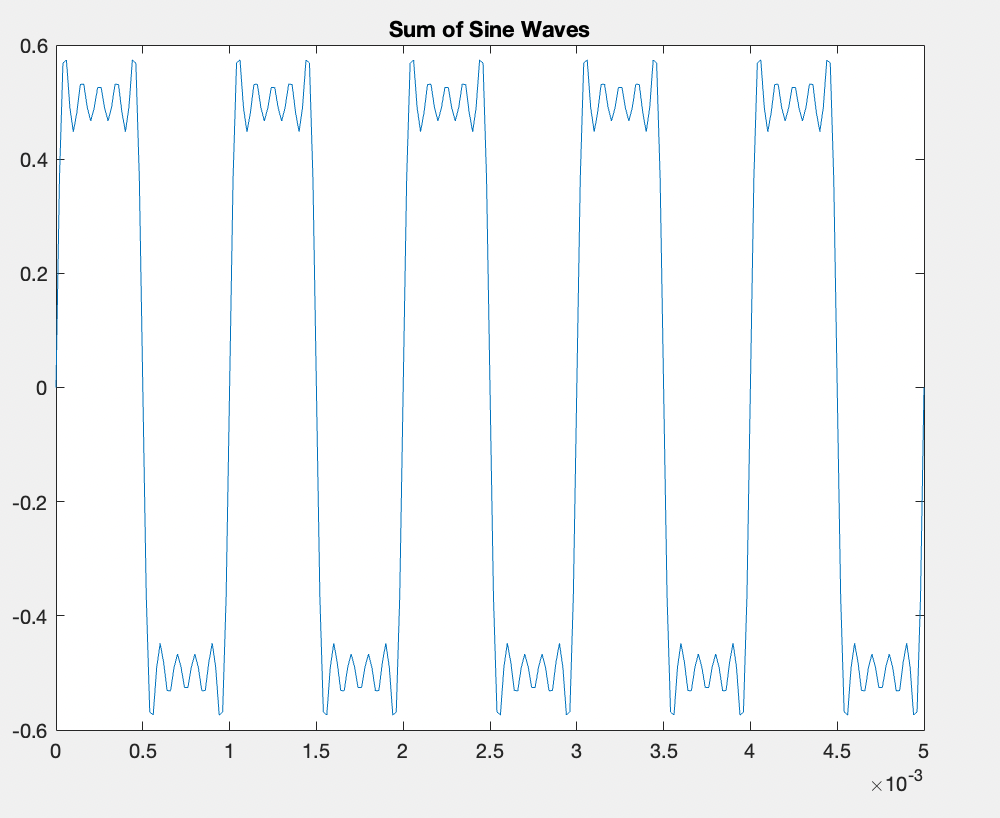
\includegraphics[width=.9\textwidth]{Figures/L7Sum2.png}
  \caption{Summing $n=1,2,3$}
  \label{fig:5}
\end{figure}

\subsection{Q13} Whereas a pure sinusoid simply sounds like a single tone, the summed sinusoids seem to resonate a bit, as, when it hits the ``bumpy'' peaks, the noise varies.

\section{Part IV}

\begin{figure}[H]
  \centering
  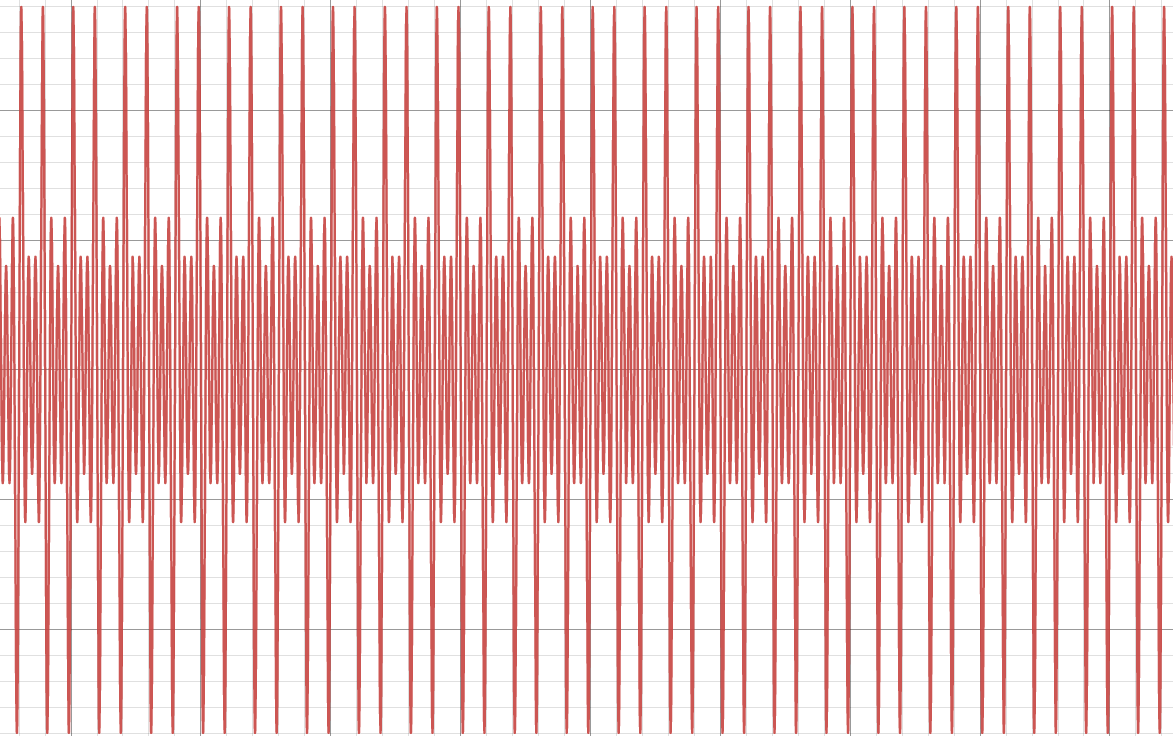
\includegraphics[width=.9\textwidth]{Figures/L7P41.png}
  \caption{Summing weighting different from $\frac{2}{(2n-1)\pi}$}
  \label{fig:6}
\end{figure}

\subsection{Q14} It seems that the wave becomes ``sharper'', as it becomes a bit more triangular, with steep falls from peaks, as shown below in Figure \ref{fig:7}.

\begin{figure}[H]
  \centering
  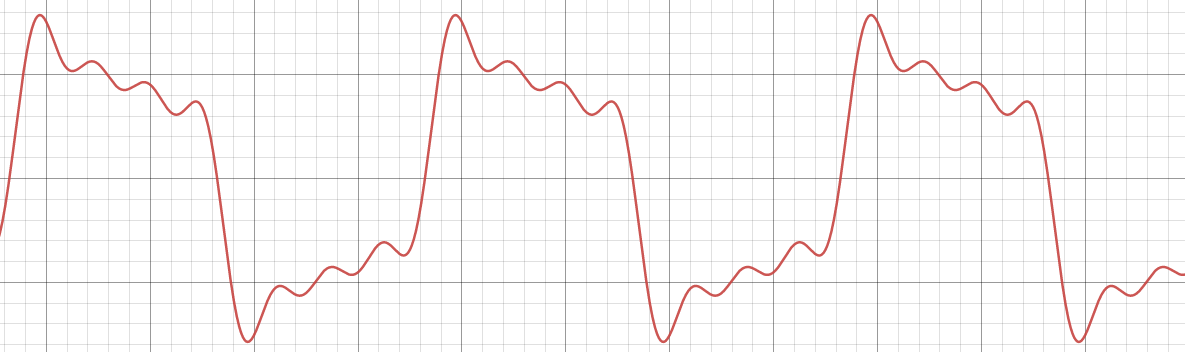
\includegraphics[width=.9\textwidth]{Figures/L7P42.png}
  \caption{The peaks become ``sharp''}
  \label{fig:7}
\end{figure}

\section{Conclusion}

Overall, this laboratory experiment allowed us to develop a rudimentary knowledge of fabrication and combination of sinusoids in the MATLAB environment; in doing so, the idea of alternating current was reinforced, as alternating current itself is a sinusoid.

\end{document}
